\section{Results}
\label{sec:results}

\subsection{The unconditional agreement, and why it is a confound}
Across $1000$ game--level pairs the two meters agree almost perfectly:
$\rho_S(\EPR,\R)=0.9927$ $[0.9914,0.9936]$. Taken alone this is the result a less careful
design would report. It is a confound. Each meter is separately near-perfectly monotone in
the harmonic fraction: $\rho_S(\EPR,\alpha)=0.9904$ and $\rho_S(\R,\alpha)=0.9819$
($n=2000$). The unconditional correlation is therefore substantially the correlation of two
functions of $\alpha$ with each other, and says nothing about whether they carry independent
information.

\subsection{Conditional on $\alpha$, the co-movement collapses}
\label{sec:collapse}
Stratifying by $\alpha$ level (Table~\ref{tab:collapse}, Figure~\ref{fig:collapse}a) the
within-level association is strong and flat for $\alpha\le0.65$, degrades over the top three
levels, and at this action count crosses zero into negative territory at $\alpha=0.95$. The
crossing is scoped: Section~\ref{sec:robustness} shows that the \emph{collapse} reproduces
at every action count tested while the \emph{negative sign} does not, so it is the collapse
and not the reversal that carries the two-coordinate claim.

\begin{table}[H]
\caption{Within-$\alpha$-level Spearman association between dissipation and response
asymmetry. $100$ games per level, $\lambda=1.2$, $N=2$, $m=3$.}
\label{tab:collapse}
\small
\begin{tabular}{lcccccccccc}
\toprule
$\alpha$ & 0.05 & 0.15 & 0.25 & 0.35 & 0.45 & 0.55 & 0.65 & 0.75 & 0.85 & 0.95 \\
\midrule
$\rho_S(\EPR,\R)$ & 0.882 & 0.812 & 0.856 & 0.849 & 0.800 & 0.870 & 0.801 & 0.610 & 0.323 & $-0.355$ \\
$\rho_S(\EPR,\|\chi-\chi^{\top}\|_F)$ & 0.768 & 0.749 & 0.823 & 0.808 & 0.757 & 0.857 & 0.792 & --- & --- & $-0.368$ \\
\bottomrule
\end{tabular}
\end{table}

\noindent\textbf{H1 is accepted.} The decline over the top three levels is monotone and the
terminal value is negative at $m=3$; the decline itself is confirmed at every $m$ tested in
Section~\ref{sec:robustness}.

\subsection{The repair hypothesis is refuted by its own test}
$\R$ is a ratio of norms, so the natural explanation of the collapse is that the denominator
$\|\chi+\chi^{\top}\|_F$---a measure of the \emph{symmetric} response, which grows with
$\alpha$---contaminates the numerator's signal. This was registered as H2a before the test:
if true, the numerator alone should retain co-movement with $\EPR$ at high $\alpha$.

It does not. The numerator alone reaches $\rho_S=-0.368$ at $\alpha=0.95$
(Figure~\ref{fig:collapse}a, dashed red), tracking the ratio almost exactly through the
collapse. \textbf{H2a is not supported}, and the consequence is the paper's central claim:
\emph{no renormalisation of the response matrix recovers the dissipation ordering at high
$\alpha$.}

H2b---that $\R$'s within-level variation becomes denominator-driven---\textbf{is accepted}:
$\rho_S(\R,1/\|\chi+\chi^{\top}\|_F)$ rises monotonically from $-0.082$ at $\alpha=0.05$ to
$0.955$ at $\alpha=0.95$ (Figure~\ref{fig:collapse}b). So the mechanism by which $\R$ loses
contact with dissipation is identified---at high $\alpha$ the ratio is measuring residual
symmetric response rather than asymmetry---but identifying it does not repair it, because
the numerator has lost contact too.

\begin{figure}[H]
\centering
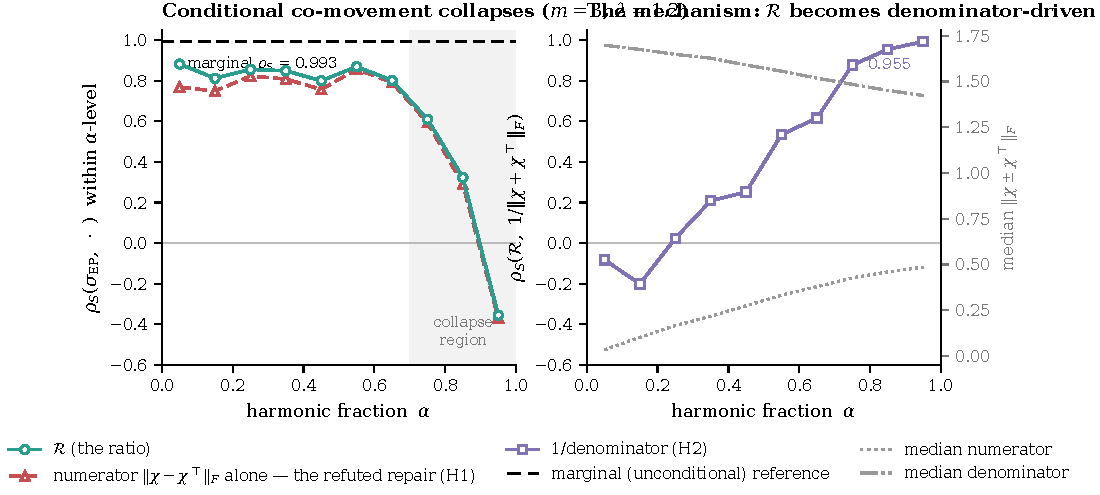
\includegraphics[width=\linewidth]{figures/fig3_collapse.pdf}
\caption{(\textbf{a}) Within-level association between dissipation and response asymmetry
against harmonic fraction, with the unconditional value as a reference. (\textbf{b}) The
mechanism, and the two norms that produce it. The refuted repair hypothesis is the dashed
red series in (\textbf{a}); by construction it would have to lie above the teal series for
H2a to hold.}
\label{fig:collapse}
\end{figure}

\subsection{The plane, and where measured systems sit in it}
Figure~\ref{fig:plane} plots both coordinates together. The synthetic $\alpha$-family runs
up the diagonal, which is what a one-dimensional theory of distance-from-equilibrium
predicts and is the reason the confound is so persuasive. The measured systems do not lie on
it. A retail scanner panel reads $\R=0.0011$ $[4.8\times10^{-5},5.0\times10^{-3}]$
($n=22{,}655$ store-weeks over $86$ stores, cluster bootstrap)---potential-like, exactly
where a single-retailer category-management model predicts, a prediction registered before
the run. A wholesale electricity day-ahead market reads $\approx1.07$ nats/day against a
reversibilized-Markov null ($p<0.01$) while sitting at null against Fourier and
amplitude-adjusted surrogates. \textbf{Those two readings fall in different quadrants}, and
each currently has only one coordinate measured---which the figure shows as a band rather
than a point.

\begin{figure}[H]
\centering
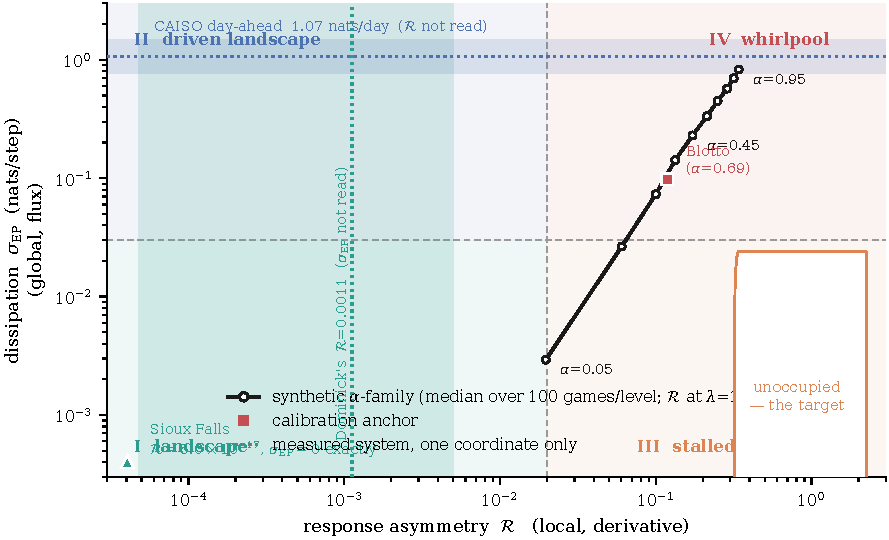
\includegraphics[width=\linewidth]{figures/fig2_plane.pdf}
\caption{The irreversibility plane. Quadrant shading uses the library's calibrated bands.
Bands rather than points indicate a system for which only one coordinate has been read.}
\label{fig:plane}
\end{figure}

\subsection{Criticality escape and the frontier}
The same operator $(I-SB)$ that gives the response also certifies uniqueness, and its
spectral radius locates the transition. On potential games $\rho(SB)$ is \emph{non-monotone}
in $\lambda$: it rises, peaks, and falls, because equilibrium concentration kills the choice
covariance faster than $\lambda$ amplifies it. Potential games therefore escape criticality
at high precision. A crossing of $\rho(SB)=1$ exists only for $\alpha\ge0.55$, and above that
the critical precision descends monotonically---$\lambda_c=7.77,\,5.22,\,4.22,\,3.64,\,3.23,\,2.95$
for $\alpha=0.55$ to $0.80$, single crossing verified at every level, zero monotonicity
violations, $n=440$ (Figure~\ref{fig:frontier}).

\begin{figure}[H]
\centering
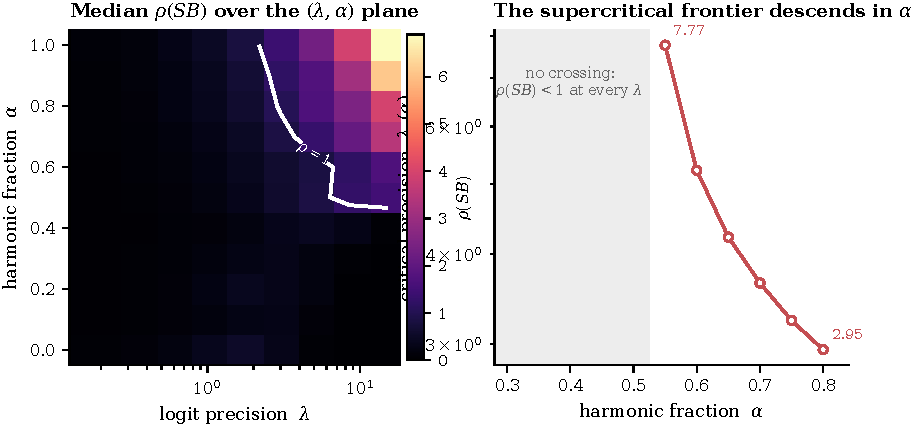
\includegraphics[width=\linewidth]{figures/fig4_frontier.pdf}
\caption{(\textbf{a}) Median spectral radius of $SB$ over the precision--harmonicity plane,
with the unit contour. (\textbf{b}) The critical precision, which exists only above
$\alpha\approx0.55$.}
\label{fig:frontier}
\end{figure}

\subsection{The dissipation axis is observable}
Against the exact meter, the $k$-block KLD estimator attains rank correlation $1.0$ across
the $\alpha$ sweep, and the debiased finite-time thermodynamic-uncertainty bound lies below
the exact value at every level with median tightness $0.850$
(Figure~\ref{fig:observability}). The bound, not the point estimate, is the reportable
statement on real data.

\begin{figure}[H]
\centering
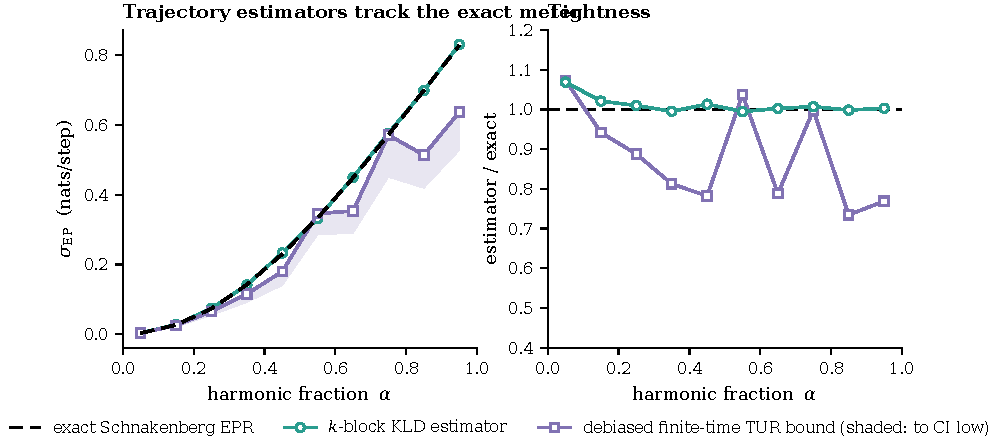
\includegraphics[width=\linewidth]{figures/fig5_observability.pdf}
\caption{(\textbf{a}) Trajectory estimators against the exact entropy production.
(\textbf{b}) Tightness. By construction the certified bound cannot exceed the exact value.}
\label{fig:observability}
\end{figure}

\subsection{Sensitivity: what is universal and what is not}
Repeating the stratified sweep across $\lambda\in\{0.8,1.2,2.0\}$ and $m\in\{3,4\}$
separates two things that a single run conflates. \textbf{The collapse is universal}: the
conditional association degrades at every setting tested. \textbf{The sign of the residual
is not}: it runs $+0.25\to+0.03\to-0.23$ as $\lambda$ increases, and
Section~\ref{sec:robustness} adds $m$ to the list of things it varies with. \textbf{H3 is
accepted; H3b is not supported.} We therefore report the existence of a second dimension as the
result, and the direction of its tilt as a system-specific property and an open question.
This distinction was not anticipated; a registered criterion failed $2$ of $4$ cells and was
revised on the record rather than quietly, and a follow-on ``wedge-depth'' explanation for
the reversal was refuted ($0$ of $180$ games supercritical).

\subsection{Two pre-registered kill-shots}
\label{sec:robustness}
The two most plausible ways the two-coordinate claim is wrong are that the collapse is
small-system noise that recovers as the action set grows (H5), and that it is an artefact of
the fixed-point solver (H6). Both were registered with their thresholds in a configuration
file committed before the experiment implementing them existed, and both have been run:
$5200$ distinct games ($6000$ solves) at $N=2$, $\lambda=1.2$, $200$ games per main cell,
percentile bootstrap ($2000$ resamples) on every reported $\rho_S$. The seed stream was reconstructed from the
reference run, so the first $100$ games of every $m=3$ cell are literally the games behind
Table~\ref{tab:collapse}; the replication deviation at $\alpha\in\{0.85,0.95\}$ is $0.000$,
which makes every comparison below anchored to the published reading rather than to a fresh
sample of it.

\begin{table}[H]
\caption{Finite-size sweep (H5). Within-level Spearman association at each action count,
$200$ games per cell, $N=2$, $\lambda=1.2$, fixed Frobenius payoff scale. Brackets are
$95\%$ percentile-bootstrap intervals; $\mathrm{gap}=\rho_S(0.05)-\rho_S(0.95)$.}
\label{tab:finitesize}
\small
\begin{tabular}{lccccccc}
\toprule
$m$ & $\alpha{=}0.05$ & $0.45$ & $0.75$ & $0.85$ & $\alpha{=}0.95$ $[95\%$ CI$]$ & gap & gap ratio \\
\midrule
3 & $+0.851$ & $+0.869$ & $+0.627$ & $+0.398$ & $-0.352$ $[-0.473,-0.226]$ & $1.203$ & $1.000$ \\
4 & $+0.806$ & $+0.773$ & $+0.685$ & $+0.438$ & $-0.272$ $[-0.405,-0.140]$ & $1.078$ & $0.896$ \\
5 & $+0.702$ & $+0.741$ & $+0.654$ & $+0.439$ & $-0.244$ $[-0.377,-0.097]$ & $0.947$ & $0.787$ \\
6 & $+0.716$ & $+0.698$ & $+0.607$ & $+0.388$ & $+0.012$ $[-0.137,+0.156]$ & $0.704$ & $0.585$ \\
\bottomrule
\end{tabular}
\end{table}

\noindent\textbf{H5 is \textsc{indeterminate}, and the reason is a criterion substitution we
report on the record.} This unit has \emph{two} registrations of the same kill-shot. The
first (\texttt{plane\_finite\_size.yaml}, committed 23:02:25) adjudicates the raw recovery
$\Delta\rho_{\mathrm{hi}}=\rho_S(6,0.95)-\rho_S(3,0.95)$: refutation iff
$\Delta\rho_{\mathrm{hi}}>0.40$, survival iff $\Delta\rho_{\mathrm{hi}}\le0.20$. An
experiment implementing it was written at 23:04:39, executed at 23:04:49, and run again at
23:17:47. The second (\texttt{plane\_robustness.yaml}, committed 23:26:36---\emph{after}
both of those runs) replaces the deciding statistic with the gap ratio
$\mathrm{gap}(6)/\mathrm{gap}(3)$ against a $0.50$ bar. On the data of
Table~\ref{tab:finitesize} the two registrations disagree, and the change ran in the
direction of survival: $\Delta\rho_{\mathrm{hi}}=+0.364$ is neither above $0.40$ nor at or
below $0.20$, so the first registration returns \textbf{indeterminate}, while the gap ratio
is $0.585$, above its bar, so the second returns survival. Both files define
\emph{indeterminate} as a third outcome for exactly this situation. Where two registrations
of one criterion disagree and the earlier was live when the data were first produced, the
earlier binds: \textbf{H5 is indeterminate}, and the claim's status under it is unchanged
rather than strengthened.

\noindent\textbf{The deciding statistic reached adjudication without an interval, and its
interval crosses the bar.} The second registration required bootstrap intervals on every
reported $\rho_S$, and stated the principle that a point estimate on the right side of a
threshold whose interval crosses it does not certify survival. The gap ratio is not a
$\rho_S$, so it received no interval. Bootstrapped after the fact ($4000$ resamples,
games resampled within cell, both $\alpha$ cells resampled per replicate, $m=3$ as the
shared denominator), $\mathrm{gap}(6)/\mathrm{gap}(3)=0.585$ with $95\%$ interval
$[+0.434,+0.749]$ and $P(\text{gap ratio}<0.50)=0.129$---a
margin of $1.08$ bootstrap standard deviations. The interval crosses $0.50$. By the
registration's own principle the surviving branch is not certified, which is a second and
independent route to the same verdict. Two of the three refutation conditions did fire:
$\rho_S$ at $\alpha=0.95$ rises with $m$ with no dip
($-0.352\to-0.272\to-0.244\to+0.012$), and the terminal intervals at $m=3$ and $m=6$ are
disjoint.

\noindent\textbf{What is robust, and what the claim rests on, is the ceiling.} The
high-$\alpha$ association never recovers to coupled behaviour at any tested action count:
$\rho_S(m,0.95)\le0.35$ at every $m$, and the \emph{upper} interval endpoint is below the
ceiling at every $m$---worst $+0.156$ against $0.35$. The $\alpha=0.05$ and $\alpha=0.95$
intervals are disjoint at every $m$, and the precondition $\rho_S(m,0.05)\ge0.55$ holds
throughout. That is what two-coordinate independence requires, and unlike the gap ratio it
is not a near thing. It is also \emph{immune to the substitution}: the $0.35$ ceiling and its
interval form are identical in both registrations---and are themselves inherited from an
earlier unit's registered collapse threshold rather than chosen here---so whichever
registration binds, this condition reads the same way and passes with room. The substitution
moved the primary statistic and nothing else. No indeterminacy guard fired: zero near-critical games, zero
non-convergences and zero generator rejections across all $6000$ solves; the verdict above
is a criterion outcome, not a data-quality one. The $m=3$ row is a re-execution of the
reference cells on the identical games, deviation $0.000$, which is the strongest single
property of the run and is independent of every criterion dispute in it.

\noindent\textbf{The sign is scoped, and the scope is narrower than we first wrote it.}
At $m=6$ and fixed Frobenius scale the terminal association in
Table~\ref{tab:finitesize} is $+0.012$ $[-0.137,+0.156]$, and an earlier version of this
section called that ``statistically indistinguishable from zero'' and concluded that the
sign reversal does not survive $m$. \textbf{That conclusion was too strong and is corrected
here.} A later run repeats the $m$-sweep at $n=400$ with a \emph{paired} control that fixes
the median normalised precision $\bar\lambda$ by construction rather than letting it drift
(Table~\ref{tab:c1b}). Two things move the number: doubling $n$ (the $+0.012$ at $n=200$
and $-0.112$ at $n=400$ are the same games plus $200$ more, and each lies inside the
other's interval---resolution, not contradiction), and holding $\bar\lambda$ fixed, which
the main arm does not.

\begin{table}[H]
\caption{The $m$-sweep repeated \emph{paired} at matched normalised precision, $400$ games
per cell, $\alpha=0.95$. The main arm's $\bar\lambda$ falls $1.855\to1.268$ across $m$; the
matched arm holds it at $1.86$--$1.91$ by construction.}
\label{tab:c1b}
\small
\begin{tabular}{lccc}
\toprule
$m$ & matched scale & matched $\rho_S$ $[95\%$ CI$]$ & fixed-scale $\rho_S$ $[95\%$ CI$]$ \\
\midrule
3 & $2.0000$ & $-0.3325$ $[-0.423,-0.246]$ & $-0.3325$ $[-0.424,-0.235]$ \\
4 & $2.3535$ & $-0.2966$ $[-0.387,-0.204]$ & $-0.2536$ $[-0.340,-0.161]$ \\
5 & $2.6308$ & $-0.2554$ $[-0.345,-0.160]$ & $-0.1760$ $[-0.268,-0.081]$ \\
6 & $3.0171$ & $\mathbf{-0.2061}$ $[-0.300,-0.105]$ & $-0.1119$ $[-0.214,-0.016]$ \\
\bottomrule
\end{tabular}
\end{table}

\noindent At matched precision the $m=6$ interval \emph{excludes} zero and the sign
reversal survives to $m=6$. Of the fixed-scale drift in the terminal association from $m=3$
to $m=6$---$+0.221$ in total---$+0.126$ survives matching and $+0.095$ is temperature. The
supported statement is therefore: at fixed Frobenius scale the reversal weakens with $m$;
at matched $\bar\lambda$ it does not. \emph{None of this changes what the paper claims.}
The claim is the weaker and sufficient one---\emph{the coupling collapses at high
$\alpha$}, with the terminal upper interval endpoint under the ceiling at every $m$---and
independence requires decorrelation, not anti-correlation. The sign reversal is retained
only with its $(m,\lambda,N)$ scope attached.

\subsection{Kill-shot three: does the plane survive more than two players?}
\label{sec:nplayers}
The limitation the previous version of this paper named as its next kill-shot---everything
at $N=2$---has been run: $16{,}000$ solves over $40$ cells at $\lambda=1.2$, $400$ games
per cell, with a paired control arm that matches the median normalised precision across $N$
by construction (worst $|\bar\lambda$ ratio $-1| = 0.031$ against a registered $0.10$
tolerance). Unlike the finite-size unit, this one has exactly \emph{one} criteria file,
committed before the experiment implementing it existed---the direct operational lesson of
the substitution reported above.

\begin{table}[H]
\caption{$N$-scaling at $m=3$, $\alpha=0.95$ and $\alpha=0.05$, matched-precision arm.
$400$ games per cell; $\mathrm{gap}=\rho_S(0.05)-\rho_S(0.95)$.}
\label{tab:nplayers}
\small
\begin{tabular}{lcccc}
\toprule
$N$ & $\bar\lambda(0.05)$ & $\rho_S(\alpha{=}0.05)$ $[95\%$ CI$]$ & $\rho_S(\alpha{=}0.95)$ $[95\%$ CI$]$ & gap $[95\%$ CI$]$ \\
\midrule
2 & $1.960$ & $+0.8469$ $[+0.810,+0.878]$ & $-0.3325$ $[-0.418,-0.232]$ & $+1.179$ $[+1.085,+1.273]$ \\
3 & $1.976$ & $+0.3776$ $[+0.290,+0.459]$ & $+0.0703$ $[-0.028,+0.163]$ & $+0.307$ \\
4 & $1.958$ & $+0.1715$ $[+0.072,+0.264]$ & $-0.0089$ $[-0.105,+0.086]$ & $+0.180$ \\
\bottomrule
\end{tabular}
\end{table}

\noindent\textbf{The refutation branch never came close.} It required
$\rho_S(\alpha{=}0.95)>0.35$ with its lower interval endpoint also above $0.35$ at some
$N>2$; the worst upper endpoint measured is $+0.163$. On the ceiling alone the plane looks
\emph{more} like a plane at $N>2$ than at $N=2$.

\noindent\textbf{But the registered precondition fails, and that is the finding.} The
criterion required $\rho_S(\alpha{=}0.05)\ge0.55$---a baseline coupling for the collapse to
be a departure \emph{from}. At matched precision it reads $+0.847$, $+0.378$, $+0.172$
across $N=2,3,4$, and the full $\alpha$ profile at $N\ge3$ is small at \emph{every} level.
A size with no baseline coupling has no collapse to measure, so the verdict is
\textbf{indeterminate}, and we decline to read absence-of-coupling-everywhere as
confirmation of two coordinates. Two rival explanations were registered in advance and both
are excluded: it is not temperature, because the matched arm fixes $\bar\lambda$ at
$1.96$--$1.98$ across $N$ and matching moves $\rho_S(0.05)$ only from $+0.282$ to $+0.378$
at $N=3$; and it is not meter degeneracy, because at matched precision both meters retain
comparable magnitudes across $N$ (median $\EPR$ $1.20/1.26/1.21\times10^{-3}$ at
$\alpha=0.05$; median $\R$ $0.0187/0.0103/0.0054$), with median distance to criticality
$0.48$--$0.94$ everywhere.

\noindent\textbf{What this does to the paper.} The claim is unchanged at $N>2$ and is not
certified there. What is narrowed is the \emph{evidence}: the $\alpha$-stratified collapse
--- the design that makes this paper persuasive, and the source of every number in
Sections~\ref{sec:collapse}--\ref{sec:robustness} --- is a \textbf{two-player instrument}.
A plausible structural reason, stated as a hypothesis with its test rather than as a
result: at $N=2$ there is exactly one non-trivial multi-player Hodge sector, so a single
harmonic modulator drives both meters; at $N=3$ there are four and at $N=4$ eleven, and the
two functionals weight them differently. The test is a regression of per-game $\R$ and
$\EPR$ on the per-sector harmonic norms at $N=3$, which the existing machinery can produce
in one pass and which has not been run.

\noindent\textbf{The same run strengthens the paper on the other axis.} The
ratio-artefact objection of Section~3.3 was re-tested on the numerator alone across
$m\in\{3,4,5,6\}$ at $N=2$ with the ratio computed on the \emph{identical} games:
$\rho_S(\EPR,\|\chi-\chi^{\top}\|_F)$ at $\alpha=0.95$ is negative with a negative
upper interval endpoint at every $m$ in both arms (worst $-0.007$), its precondition holds
at every $m$, and the paired difference between the numerator and the ratio is bounded by
$0.012$ and shrinks with $m$. Removing the denominator changes the rank ordering against
$\EPR$ by less than one part in eighty---a paired bound where the original refutation had
only a point estimate.

\noindent\textbf{H5b: the onset does not drift.} The smallest swept level at which
$\rho_S<0.5$ is $\alpha=0.85$ at every $m\in\{3,4,5,6\}$---drift $0.00$ against a tolerance
of $0.10$. Where the collapse begins is $m$-independent; only how far it goes at
$\alpha=0.95$ moves with $m$, and, as the next paragraph shows, only at fixed Frobenius
scale.

\subsubsection{The $m$-trend is largely, not wholly, a normalised-precision effect}
The generator unit-normalises each Hodge component and multiplies by a fixed Frobenius
scale, so per-entry payoff RMS falls like $1/m$: a larger action set is also a
\emph{colder} game. Across the main sweep at $\alpha=0.95$ the median normalised precision
$\bar\lambda=\lambda\cdot(\text{payoff range})$ falls $1.86\to1.62\to1.42\to1.27$ and the
median $\EPR$ falls $0.546\to0.318\to0.206\to0.144$ as $m$ goes $3\to6$. The registered
control D1 repeats the extreme levels under the a-priori rule
$\text{scale}(m)=2.0\,m/3$, which holds per-entry RMS approximately constant
($\bar\lambda=1.85\to2.18\to2.38\to2.58$):

\begin{table}[H]
\caption{Payoff-scale control (D1), registered before the run. $100$ games per
cell, same levels, same $\lambda$. The control raises $\bar\lambda$ with $m$ where the main
arm lowers it, so the two arms \emph{bracket} the confound rather than matching it.}
\label{tab:d1}
\small
\begin{tabular}{lcccc}
\toprule
$m$ & $\rho_S(\alpha{=}0.05)$ & $\rho_S(\alpha{=}0.95)$ $[95\%$ CI$]$ & $\bar\lambda(\alpha{=}0.95)$ & gap ratio \\
\midrule
3 & $+0.852$ & $-0.347$ $[-0.516,-0.170]$ & $1.85$ & $1.000$ \\
4 & $+0.625$ & $-0.431$ $[-0.584,-0.251]$ & $2.18$ & $0.881$ \\
5 & $+0.779$ & $-0.453$ $[-0.617,-0.258]$ & $2.38$ & $1.027$ \\
6 & $+0.747$ & $-0.300$ $[-0.471,-0.116]$ & $2.58$ & $0.872$ \\
\bottomrule
\end{tabular}
\end{table}

\noindent In the control arm the terminal association is non-monotone in $m$, the negative
sign is intact at every $m$ including $m=6$, and the collapse at $m=6$ retains $87\%$ of its
$m=3$ size instead of $59\%$ (Figure~\ref{fig:robustness}b). \textbf{This does not mean the
$m$-trend vanishes at matched effective precision, and we withdraw that reading.} D1 does
not hold $\bar\lambda$ constant: it drives $\bar\lambda$ \emph{up} $40\%$ across
$m\in\{3,\dots,6\}$ ($1.85\to2.58$) where the main arm drives it \emph{down} $32\%$
($1.86\to1.27$). The two arms therefore bracket the confound rather than controlling it, and
the honest reading is an interpolation between them: taking $\rho_S(6,0.95)$ linearly in
$\bar\lambda$ between the two arms and evaluating at the $m=3$ arms' common
$\bar\lambda\approx1.86$ gives $\approx-0.13$, leaving a residual $m$-effect of $\approx0.22$
of the observed $0.364$. \textbf{Most of the $m$-effect survives matching.} The supported
statement is that the apparent finite-size decay is \emph{largely, not wholly}, a
normalised-precision effect of the game generator, consistent with this programme's earlier
results on the $\lambda$-sensitivity of both meters. Both arms return the same verdict under
the second registration, so the registered disagreement rule does not fire; but D1 is
\emph{unpaired} to the main arm---a different seed offset and half the games per cell---so
every arm-to-arm comparison here carries between-sample noise a paired design would cancel,
and the control should be re-run paired at $\bar\lambda$ fixed by construction. The
methodological consequence stands and is restated among the limitations in
Section~\ref{sec:discussion}: an $m$-sweep on this family that does not control per-entry
payoff RMS will confound temperature with dimension.

\subsubsection{The collapse is not numerical, and the solver check is a diagnostic}
\textbf{H6 returns $|\Delta\rho_S|=0.00000$, and that number had no way to come out
otherwise.} At $m=3$, on the identical $100$-game families at $\alpha\in\{0.85,0.95\}$,
magnetic mirror descent and the damped solver at a $100\times$ tighter tolerance both
reproduce the reference association exactly, in all four comparisons, against a registered
bar of $0.05$. The supporting diagnostics say why: the maximum sup-norm deviation in the
equilibrium mixture is $2.7\times10^{-12}$ and the maximum deviation in $\R$ itself is
$1.3\times10^{-12}$. $\rho_S$ is a \emph{rank} statistic, and a perturbation twelve orders of
magnitude below the spacing of adjacent $\R$ values in a $100$-game sample cannot reorder
them; $|\Delta\rho_S|=0$ was therefore arithmetically forced before the run rather than
discovered by it, and its ``margin'' against the $0.05$ bar is not evidence. We report H6 as
what it actually measures---\textbf{the solver contributes $\sim\!10^{-12}$ to $\R$, and the
rank ordering of $\R$ is bit-stable under solver replacement}---which is a real result and
excludes finite-precision path dependence, the stated H6 hypothesis. It is not a kill-shot
passed with margin. A test with power would have to perturb $\R$ at the scale of the rank
spacing, or use a statistic sensitive to magnitude. Since $\EPR$ is computed from the
generator and never touches the solver, the solver can enter this correlation only through
$\R$; and no comparison of two methods converging to the same fixed point can exclude a bias
shared by both.

\begin{figure}[H]
\centering
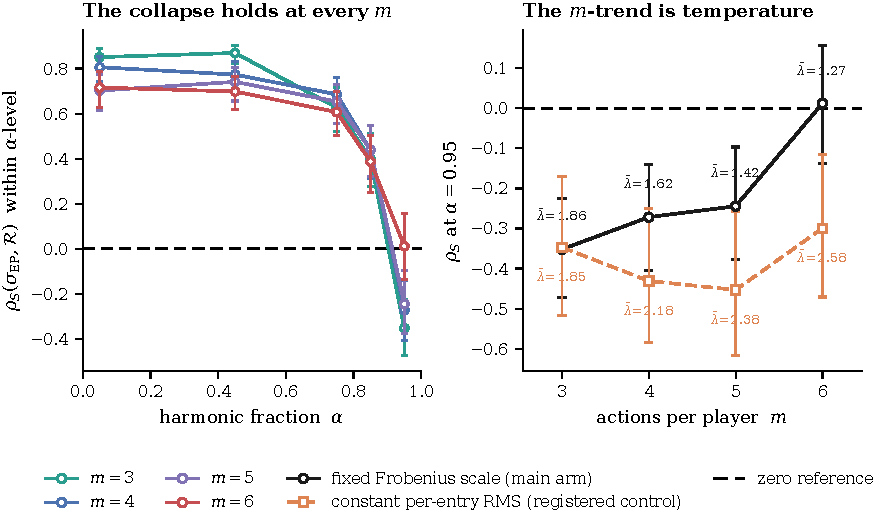
\includegraphics[width=\linewidth]{figures/fig6_robustness.pdf}
\caption{(\textbf{a}) Within-level association against harmonic fraction at each action
count, with bootstrap intervals and the zero reference. (\textbf{b}) The terminal
association at the highest swept level under fixed Frobenius payoff scale against the
registered constant-per-entry-RMS control, annotated with the median normalised precision
each arm actually ran at.}
\label{fig:robustness}
\end{figure}

\subsection{Calibration}
Both meters read zero where zero is provably correct, on data the project did not generate.
Sioux Falls road network: $\R=5.6\times10^{-17}$, Fisk stochastic-user-equilibrium KKT
spread $7.1\times10^{-15}$, directional-derivative symmetry defect exactly $0$. A degenerate
equal-value Blotto instance: $\EPR=5.4\times10^{-32}$. Colonel Blotto at budget $3$:
$\alpha=0.694$, $\R=0.118$; rock--paper--scissors: $\R\approx0.69$--$0.87$.

\subsection{Hypothesis scoreboard}
\begin{table}[H]
\caption{Registered hypotheses and outcomes. Criteria and levels were fixed before the runs.}
\label{tab:scoreboard}
\footnotesize
\setlength{\tabcolsep}{3.4pt}
\begin{tabular}{llll}
\toprule
\textbf{Hypothesis} & \textbf{Criterion} & \textbf{Result} & \textbf{Outcome} \\
\midrule
H1 conditional decline & monotone over top 3 levels ($m{=}3$) & $0.610\to0.323\to-0.355$ & Accepted \\
H2a ratio artefact & numerator $\rho_S>0.5$ at high $\alpha$ & $-0.368$ & \textbf{Not supported} \\
H2b denominator-driven & $\rho_S>0.8$ at high $\alpha$ & $0.955$ & Accepted \\
H3 collapse universal & degrades at every $(\lambda,m)$ & holds $3\times2$ cells & Accepted \\
H3b sign $\lambda$-invariant & same sign across $\lambda$ & $+0.25/+0.03/-0.23$ & \textbf{Not supported} \\
H4 observable on real data & both coordinates, no payoffs & one coordinate each, 2 systems & Partly accepted \\
\midrule
\multicolumn{4}{l}{\emph{Kill-shots, registered before the experiment existed}}\\
H5 finite size, \emph{first} registration & $\Delta\rho_{\mathrm{hi}}>0.40$ / $\le0.20$ & $+0.364$: neither branch & \textbf{Indeterminate} \\
H5 finite size, \emph{replacement} & gap ratio vs $0.50$ bar & $0.585$ $[+0.434,+0.749]$, crosses bar & Survives on the point est. \\
H5 as reported & earlier registration binds & registrations disagree & \textbf{Indeterminate} \\
H5 ceiling condition & $\rho_S(m,0.95)$ CI below $0.35$ & worst $+0.156$; ends disjoint at every $m$ & \textbf{Holds; carries the claim} \\
H5, the sign half & --- & $+0.012$ $[-0.137,+0.156]$, $m{=}6$ & \textbf{Reversal not general} \\
H5b onset drift & drift $\le0.10$ in $\alpha$ & $0.00$ at every $m$ & Passed \\
H6 solver artefact & $|\Delta\rho_S|<0.05$, 4 comparisons & $0.00000$; $\R$ moved $\sim10^{-12}$ & Diagnostic, not a test \\
D1 payoff-scale control & arms must agree & agree; brackets $\bar\lambda$, does not fix it & Confound found, unpaired \\
\midrule
\multicolumn{4}{l}{\emph{Third kill-shot, one criteria file, committed before its experiment existed}}\\
H7 $N$-scaling & $\rho_S$ CI below $0.35$ at $N{\in}\{3,4\}$ & worst $+0.163$ & Ceiling holds \\
H7 precondition & $\rho_S(\alpha{=}0.05)\ge0.55$ at each $N$ & $+0.847/+0.378/+0.172$ & \textbf{Fails at $N\ge3$} \\
H7 as reported & precondition binds & no baseline to collapse from & \textbf{Indeterminate} \\
H7b onset drift in $N$ & one-sided, drift $\le+0.10$ & $-0.80$ ($0.85\to0.05$) & \textbf{Passes vacuously} \\
H8 numerator across $m$ & CI below $0.35$ at every $m$, $N{=}2$ & worst $-0.007$; paired $\delta\le0.012$ & \textbf{Holds} \\
C1 paired $\bar\lambda$ control & arms agree; $|\bar\lambda$ ratio $-1|\le0.10$ & agree; $0.031$ & Binding, satisfied \\
\bottomrule
\end{tabular}
\end{table}
